\setcounter{equation}{0}
\setcounter{figure}{0}

\section{Intro to Electromagnetic Induction}
\label{electromagnetic_induction}

\makelabheader %(Space for student name, etc., defined in master.tex)

%\textbf{Objective:}

%\begin{itemize}
%\item 
%To investigate the effect of changing magnetic fields on induced emf and current.
%\end{itemize}

\bigskip

\textbf{Introduction} 

%A charged object moving through a magnetic field experiences a force
%which is proportional to the magnitude of its charge and to its speed
%perpendicular to the field: $F = qvB_\perp$. 
If the magnetic flux through a coil of wire changes, an emf (or voltage) 
will be induced in the coil. This is Faraday's Law. If the coil of wire 
forms a closed loop, then a current will be induced in the wire. The direction 
of this current is such that the magnetic field it produces opposes the change 
in the external field. This is known as Lenz's Law. Similarly, varying the 
current in one coil (the primary) produces a current in another nearby coil 
(the secondary) due to the varying magnetic field produced by the first coil. 
The current in the second coil will flow in a direction that creates a magnetic
field which opposes the change in the field of the first coil (again, due to 
Lenz's Law). These relationships between changing fields and currents are known 
collectively as electromagnetic induction.

\bigskip

\begin{wrapfigure}[9]{r}{0.3\textwidth}
\vspace{-0.2in}
    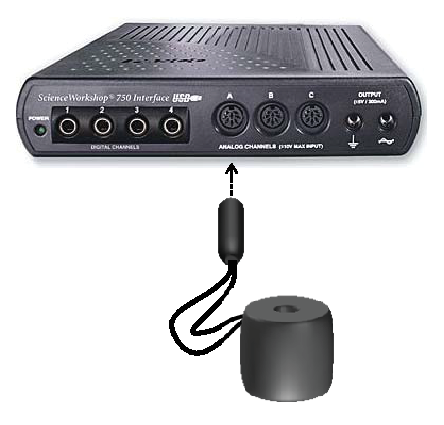
\includegraphics[width=0.3\textwidth]{induction1/induction1_setup.eps}
\end{wrapfigure}

\textbf{Apparatus}

\begin{itemize}%[nolistsep]
\setlength\itemsep{-4pt}
\setlength\topsep{-6pt}
\setlength\partopsep{-6pt}
\vspace{-0.2in}  

\item one small wire coil
\item Pasco 750 Interface with voltage sensor
\item two alligator clips
\item bar magnet
%\item Pasco 750 Interface
\end{itemize}

\textbf{Activity 1: A Moving Magnet and a Coil}

\begin{enumerate}
\setlength\rightmargin{3in}

\item Connect the coil to the voltage sensor using the alligator clips.  Connect the voltage sensor to port A on the Pasco 750 interface.
Turn on the computer and launch \textit{EM Induction} in the \textit{132 Workshop} folder under \textit{Physics Applications} in the \textbf{Start} menu.

\end{enumerate}

\vspace{-0.3in}  

\begin{enumerate}[resume]

%Ending and Resuming the enumerate environment is a kluge, which is necessary to make the enumerate environment play nicely with the wrapfig environment.  Without the ending and resuming, the changed right margin from the wrapfig persists until the end of the list.  Note that this resuming requires the ``enumitem'' package.

\item Place a bar magnet vertically along the axis of the small coil with
the north pole touching the coil.

\item Start recording data and lift the bar magnet quickly straight up.

\item At the end of the data taking interval, the computer should display
a value for the emf (the voltage) induced in the small coil.
Several trials may be required to get the correct timing between starting
the data acquisition and removing the magnet. Note and record the sign of the 
induced emf.
\answerspace{8mm}

\item \textbf{Prediction}: If you lower the magnet, north pole down, quickly
toward the coil, what will be the sign of the emf? 
\answerspace{8mm}

\item Carry out the experiment, starting the data acquisition, then lowering the magnet.
Record the sign of the induced emf.
\answerspace{8mm}

\item Did your result confirm or refute your prediction?
\answerspace{15mm}

\pagebreak[3]
\item \textbf{Prediction}: What will happen to the emf if you perform the
same pair of experiments with the south pole toward the coil? \vspace{10mm}

\item Perform the two experiments, lifting and lowering the magnet, with
the south pole down. Record the sign of the induced emf in each case.\vspace{10mm}

\item How did the results compare with your predictions?\vspace{10mm}

\end{enumerate}

\textbf{Activity 2: Predictions About Making Waves Electromagnetically}

Consider what we have observed about electricity and magnetism.
A static, unchanging magnetic field does not do much to our coil of wire.
A varying magnetic field creates, across space, a current in our coil.
The changing magnetic field must be creating an electric field or else the electrons
in the coil would not feel a force.
We have also observed phenomena where a changing electric field induced a magnetic
field.
In other words, a changing electric field induces a magnetic field and vice versa;
a changing magnetic field induces an electric field.
Notice these statements don't require the presence of electrons or other material.
The fields can be induced in a vacuum.
We are now going to explore via a simulation, what happens when  charges are wiggled
(\textit{i.e.} oscillate) up and down.

\begin{enumerate}

\item To begin to explore our wiggling charges, consider some questions.
Suppose the motion of the charges can be described as an oscillating dipole so the \
dipole moment as a function of time looks like Figure 1.
Assume the dipole is aligned with the $z$-axis.
What do you expect the electric field to look like as a function of time 
at some arbitrary distance $r$
away from the source in the $x-y$ plane?
What is the direction of the $\vec E$ field?
Make a sketch of your answer on the plot and label your curve.
\begin{figure}[hbt]
\hspace{0.375in}\includegraphics[height=2.5in]{induction1/fig1_bw.eps}
\caption{Time dependence of a dipole source oriented along the $z$-axis.}
\end{figure}

%\newpage

\item What would the magnetic field strength look like as a function of time at the same 
distance $r$ from the source?
In what direction does the $\vec B$ field point?
How are the directions of the $\vec E$ and $\vec B$ field related?
Draw a dashed line on Figure 1 to represent the magnetic field strength.
\vspace{2.0cm}

\end{enumerate}
\begin{comment}
\textbf{Activity 3: Simulating Electromagnetic Waves}

We are now going to use a computer simulation to investigate the behavior of our oscillating dipole.
The situation we are exploring is very similar to the generation of radio waves with an antenna.
Charges (usually electrons) are driven up and down in the antenna and emit electromagnetic 
waves.

\begin{enumerate}

\item Open {\it Internet Explorer} ({\it IE$~$}) and go to the website
{\tt \verb!http://www.falstad.com/emwave2!}. A Java applet will pop up showing
brightly colored waves like the ones in Figure 2 propagating outward from our oscillating
electric dipole. 
If you don't see this window, consult your instructor.
\begin{figure}[hbt]
\begin{center}
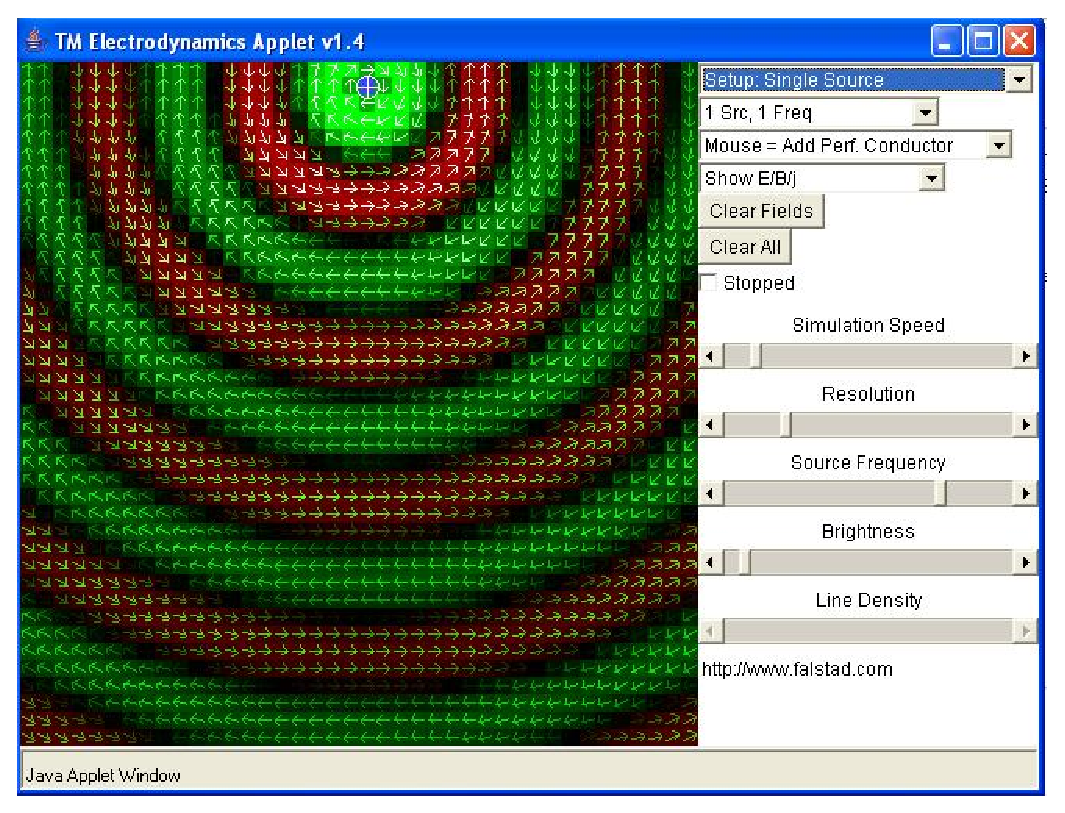
\includegraphics[width=6.0in]{induction3/emwaves1.eps}
\caption{Applet showing electromagnetic waves.}
\end{center}
\end{figure}

\item It is useful to slow down the simulation speed to observe the waves more clearly.
Do this using the slide labeled
{\tt Simulation Speed} on the right-hand side of the applet window.
The alternating yellow and blue circle at the top of the applet is the source (the dipole)
as viewed from above.
The color indicates the electric field; green areas are positive 
($\vec E$ toward you) and the red areas are negative ($\vec E$ away from you). 
The electric field is always perpendicular to the plane of the screen.
In addition to the red and green color, you will see arrows which indicate the 
direction of the magnetic field (which is always in the plane of the screen).
Also, sources and conductors may show a blue or yellow color, indicating current. 
Yellow means that current is flowing toward you and blue means it is flowing away from you. 
Describe what you see in your own words.
\vspace{3.0cm}

\item Are these waves spherical or plane waves? Why?
\vspace{1.5cm}

\item What is the orientation of the $\vec E$ field?
What is the orientation of the $\vec B$ field?
How are the two related?
\vspace{2.0cm}

\item Go back to your predictions in Activity 2 about the directions of the $\vec E$ 
and $\vec B$ fields.
Compare your predictions with these observations. Correct any disagreements.
\vspace{2.0cm}

\item Reduce the frequency of the oscillation of the dipole using the slide labeled
{\tt Source Frequency} on the right-hand side of the applet.
You may have to increase the brightness of the applet using the slide labeled
{\tt Brightness}.
What happens to the distance between equal positions on successive waves
({\it i.e.}, successive peaks or crests of the waves defined by the red regions in the
applet)?
This distance is called the wavelength and it is characteristic of a particular
wave.
Light, for example,  is an electromagnetic wave and different wavelengths correspond 
to different colors.
\vspace{2.0cm}

\item One can calculate a quantity known as the Poynting vector which points in the direction of the flow of energy in an individual wave. Make the applet draw the Poynting vector by clicking on the arrow in the box with 
{\tt Show E/B/j} entered in it. Scroll up or down until you find
{\tt Show Poynting vector} and highlight it.
In what direction does the energy flow?
\vspace{1.0cm}

\item Go back to {\tt Show E/B/j} mode you were in before. 
Just for fun, we want to introduce one of the central phenomena associated
with waves known as interference.
Go to the second menu from the top of the right-hand side of the applet.
Click and highlight {\tt 2 Src, 1 Freq}.
This will place an additional oscillating dipole at the bottom of the applet.
Describe what happens.
When waves add together they can cancel one another (this is called destructive 
interference).
Do you observe destructive interference?
What do you think happens for constructive interference?
\vspace{1.5cm}

\item Now use your mouse to grab one of the sources and drag it to a position
near the other one.
How does the interference pattern change?
Try different positions for the source (move it closer or further away).
Describe what you see.
If these were light waves, where would you see bright light?
Where would you see dark regions?
\vspace{2.0cm}

\end{enumerate}

\textbf{Activity 4: Plane Waves}

You just completed a study of spherical waves emitted by a dipole source.
We now want to consider another type of wave that we will study when we explore light.

\begin{enumerate}

\item  Use {\it IE} to go to the site
{\tt \verb!http://www.amanogawa.com/archive/PlaneWave/PlaneWave-2.html!} and a Java applet will appear 
like the one in Figure 3. 
If you don't see this window, consult your instructor.
The top panel of the applet shows a plane, electromagnetic wave.
The red lines represent the direction and magnitude of the $\vec E$ field and the
blue ones do the same for the $\vec B$ field.
NOTE: The magnetic field in this applet is labeled $\vec H$.
In this case, this is exactly the same as our previous $\vec B$.
To eliminate some unnecessary lines, click the box beside {\tt Phasors} so the check in the box 
disappears.
\begin{figure}[hbt]
\begin{center}
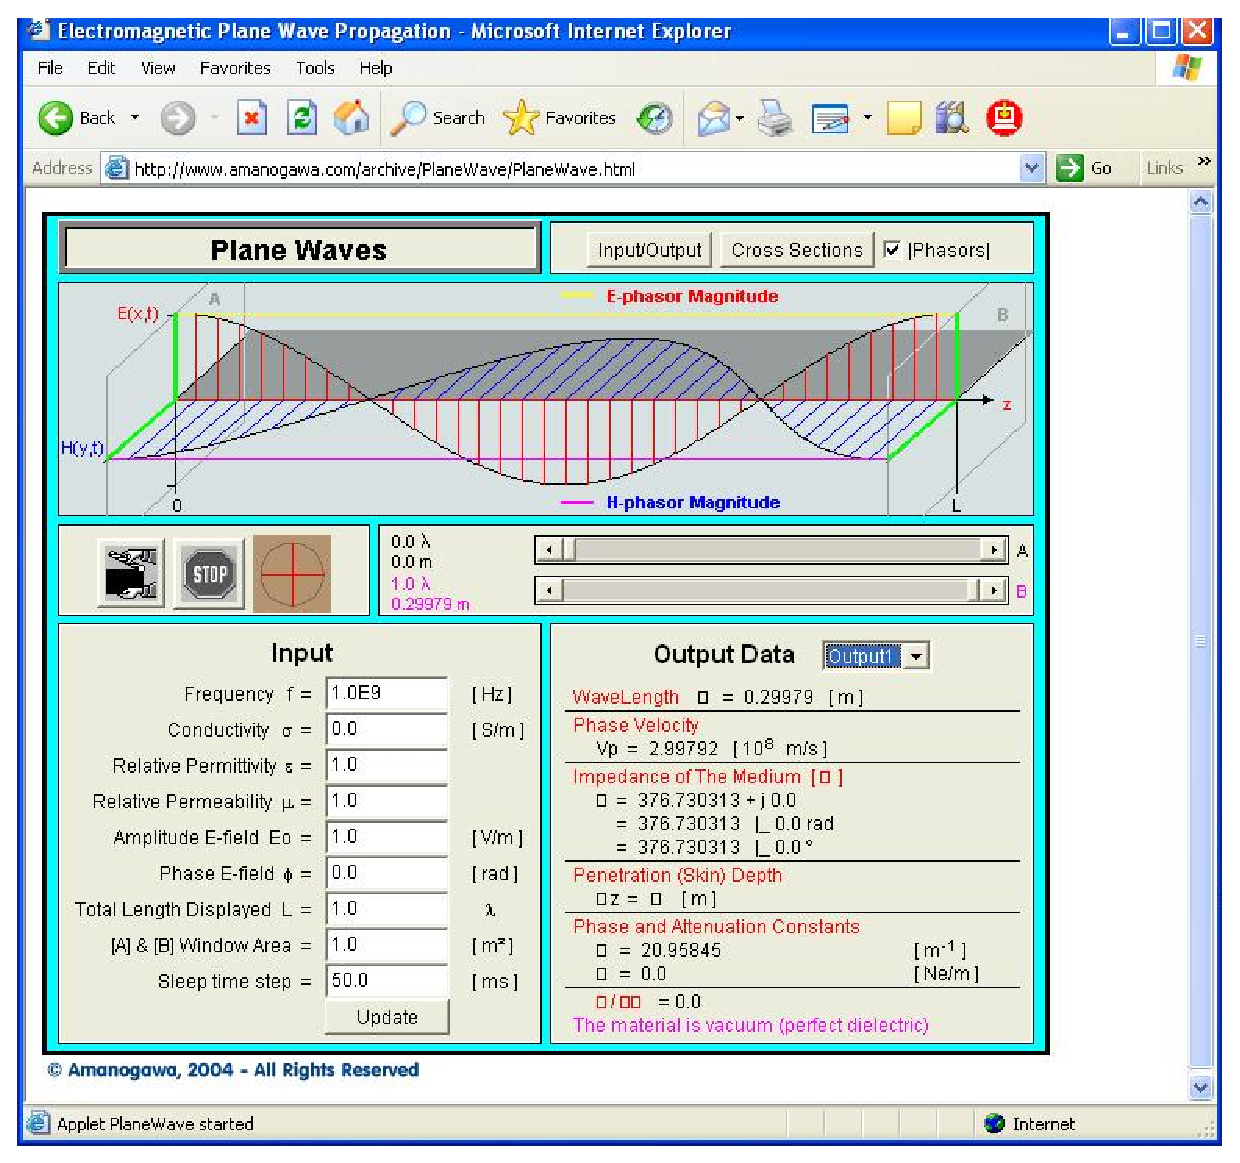
\includegraphics[width=4.0in]{induction3/emwaves3.eps}
\caption{Applet showing plane electromagnetic waves.}
\end{center}
\end{figure}

\item Why do you think it's called a plane wave?
\vspace{2.0cm}

\item What is the orientation of the $\vec E$ field?
What is the orientation of the $\vec B$ field?
Compare your answer here with your predictions in Activity 2 and your observations in part 3.4.
Correct any disagreements.
\vspace{2.0cm}

\item Click the start button to watch the wave move or propagate. The button is the one to the left of the STOP button on the top of the applet.
Describe what happens to the electric and magnetic fields and how they are related
({\it i.e.} When the $\vec E$ is large, what is the $\vec B$ field doing?).
\vspace{3.0cm}

\item Click on the {\tt Cross Sections} button at the top of the applet.
You will see new panels that show the $\vec E$ (red) and $\vec B$ (blue) vectors in cross section at the
planes $A$ and $B$ labeled in the top panel.
Use these vectors to confirm your observations in parts 4.3-4.4.
\vspace{3.0cm}

\item Use the $B$ slide at the bottom of the applet to move the $B$ cross 
section position.
Set it one-half wavelength from the $A$ cross section.
How are the $\vec E$ and $\vec B$ vectors in the $A$ cross section related to their partners 
in the $B$ cross section.
What will be the total electric and magnetic fields if two waves are added that are out of line
by one-half wavelength?
\vspace{3.0cm}

\end{enumerate}
\end{comment}
